\documentclass[12pt]{article}  

%Pachete pentru desenarea de grafuri si circuite
\usepackage[unicode]{hyperref} 
\usepackage{amsmath,epsfig,pifont,calc,pifont}	
\usepackage{tikz}
\usepackage{circuitikz}
\usetikzlibrary{shapes,arrows,positioning}
\usetikzlibrary{decorations.markings}
\usepackage{graphicx}
\usepackage{float}
\graphicspath{{images/}}
\usepackage{rom}

% Setari ale paginii / indentare
\setlength{\parindent}{3ex}
\setlength{\voffset}{-2cm}
\setlength{\textheight}{23cm}  
\setlength{\textwidth}{16cm}
\setlength{\topmargin}{0cm}
\setlength{\headsep}{1cm}
\renewcommand{\baselinestretch}{1.2}
\newcommand{\myindent}{\hspace*{3ex}}

% Margini
\setlength{\oddsidemargin}{0.5cm}
\setlength{\evensidemargin}{-0.3cm}
\raggedbottom

%Necesare; in caz contrar apare Contents, respectiv Figure
\renewcommand{\contentsname}{Cuprins}
\renewcommand{\figurename}{Figura}

%Introducem fisierul cu definitii
\makeatletter

\pgf@circ@Rlen = \pgfkeysvalueof{/tikz/circuitikz/bipoles/length}
\def\TikzBipolePath#1#2{\pgf@circ@bipole@path{#1}{#2}}
\makeatother

\newlength{\ResUp} 
\newlength{\ResRight}

%%%%%%%%%%%%%%%%%%%%%%%%%%%%%%%%%%%%%%%%%%%%%%%%%%%%%%%%%%%%%%%%%%%%%%%%%%%%%%%%%%%%%%%%%%%%%
%%%%%%%%%%%%%%%%%%      Sursa de curent: simbol folosit in Romania    %%%%%%%%%%%%%%%%%%%%%%%
%%%%%%%%%%%%%%%%%%%%%%%%%%%%%%%%%%%%%%%%%%%%%%%%%%%%%%%%%%%%%%%%%%%%%%%%%%%%%%%%%%%%%%%%%%%%%

%Declaram dimensiunile initiale
\ctikzset{bipoles/romanianCurrentSource/height/.initial=.60}
\ctikzset{bipoles/romanianCurrentSource/width/.initial=.60}

%Definim noul simbol pentru SIC
\pgfcircdeclarebipole{} 
	%Offset pentru label-uri
	{\ctikzvalof{bipoles/romanianCurrentSource/height}}
	%Numele simbolului
	{romanianCurrentSource}
	%Dimensiunile "cutiei" in care va sta
	{\ctikzvalof{bipoles/romanianCurrentSource/height}}
	{\ctikzvalof{bipoles/romanianCurrentSource/width}}
	{
		%Stabilim grosimea standard a liniei pentru un element
		\pgfsetlinewidth{\pgfkeysvalueof{/tikz/circuitikz/bipoles/thickness}\pgfstartlinewidth}
		
		%Definim ancorele
		\pgfextracty{\ResUp}{\northeast}
		\pgfextractx{\ResRight}{\southwest}
		
		%Desenam cerculetul
		\pgfpathellipse{\pgfpointorigin}{\pgfpoint{0}{\ResUp}}{\pgfpoint{\ResRight}{0}}
		
		%Desenam prima sagetica; trebuie sa avem grija ca dupa ce desenam un segment,
		%urmatoarea linie va fi desenata relativ la capatul segmentului, nu fata de
		%origine, deci sunt necesare cateva repozitionari
		\pgfmoveto{\pgfpoint{1.0\ResRight}{0.0\ResUp}}   %Ne pozitionam in (-1, 0)
		\pgflineto{\pgfpoint{0.1\ResRight}{0.0\ResUp}}   %Desenam corpul sagetii
		\pgflineto{\pgfpoint{0.3\ResRight}{-0.25\ResUp}} %Desenam unul din capete
		\pgfmoveto{\pgfpoint{0.1\ResRight}{0.0\ResUp}}   %Ne pozitionam in (-0.1, 0)
	    \pgflineto{\pgfpoint{0.3\ResRight}{0.25\ResUp}}  %Desenam celalalt capat
		
		%Desenam ce-a de-a doua sagetica
		\pgfmoveto{\pgfpoint{-0.2\ResRight}{0.0\ResUp}}  %Ne pozitionam in (0.2, 0)
		\pgflineto{\pgfpoint{-1.0\ResRight}{0.0\ResUp}}  %Desenam corpul sagetii
		\pgfmoveto{\pgfpoint{0.0\ResRight}{0.25\ResUp}}  %Ne repozitionam
		\pgflineto{\pgfpoint{-0.2\ResRight}{0.0\ResUp}}  %Desenam unul din capete
		\pgflineto{\pgfpoint{0.0\ResRight}{-0.25\ResUp}} %Desenam celalat capat
		
		%Pentru desenare, sa folosim functia draw
		\pgfusepath{draw}
	}

%Ii definim un stil si o cale si...gata!
\def\romanianCurrentSourcepath#1{\TikzBipolePath{romanianCurrentSource}{#1}}
\tikzset{romanianCurrentSource/.style = {\circuitikzbasekey, /tikz/to path=\romanianCurrentSourcepath, l=#1}}

%%%%%%%%%%%%%%%%%%%%%%%%%%%%%%%%%%%%%%%%%%%%%%%%%%%%%%%%%%%%%%%%%%%%%%%%%%%%%%%%%%%%%%%%%%%%%
%%%%%%%%%%%%%%%%%%      Sursa de ctensiune: simbol folosit in Romania    %%%%%%%%%%%%%%%%%%%%
%%%%%%%%%%%%%%%%%%%%%%%%%%%%%%%%%%%%%%%%%%%%%%%%%%%%%%%%%%%%%%%%%%%%%%%%%%%%%%%%%%%%%%%%%%%%%

%Declaram dimensiunile initiale
\ctikzset{bipoles/romanianVoltageSource/height/.initial=.60}
\ctikzset{bipoles/romanianVoltageSource/width/.initial=.60}

%Definim noul simbol pentru SIT
\pgfcircdeclarebipole{}
	%Stabilim grosimea standard a liniei pentru un element
	{\ctikzvalof{bipoles/romanianVoltageSource/height}}
	%Numele simbolului
	{romanianVoltageSource}
	%Dimensiunile "cutiei" in care va sta
	{\ctikzvalof{bipoles/romanianVoltageSource/height}}
	{\ctikzvalof{bipoles/romanianVoltageSource/width}}
	{
		%Stabilim grosimea standard a liniei pentru un element
		\pgfsetlinewidth{\pgfkeysvalueof{/tikz/circuitikz/bipoles/thickness}\pgfstartlinewidth}
		
		%Definim ancorele
		\pgfextracty{\ResUp}{\northeast}
		\pgfextractx{\ResRight}{\southwest}
		
		%Desenam cerculetul
		\pgfpathellipse{\pgfpointorigin}{\pgfpoint{0}{\ResUp}}{\pgfpoint{\ResRight}{0}}
		
		%Desenam prima sagetica; trebuie sa avem grija ca dupa ce desenam un segment,
		%urmatoarea linie va fi desenata relativ la capatul segmentului, nu fata de
		%origine, deci sunt necesare cateva repozitionari
		\pgfmoveto{\pgfpoint{1.0\ResRight}{0.0\ResUp}}   %Ne pozitionam in (-1, 0)
		\pgflineto{\pgfpoint{-1.0\ResRight}{0.0\ResUp}}   %Desenam corpul sagetii
		\pgflineto{\pgfpoint{-0.7\ResRight}{-0.25\ResUp}} %Desenam unul din capete
		\pgfmoveto{\pgfpoint{-1.0\ResRight}{0.0\ResUp}}   %Ne pozitionam in (-0.1, 0)
	    \pgflineto{\pgfpoint{-0.7\ResRight}{0.25\ResUp}}  %Desenam celalalt capat
		
		%Pentru desenare, sa folosim functia draw
		\pgfusepath{draw}
	}
	\def\romanianVoltageSourcepath#1{\TikzBipolePath{romanianVoltageSource}{#1}}
%Ii stabilim un nume, un posibil label si...gata!
\tikzset{romanianVoltageSource/.style = {\circuitikzbasekey, /tikz/to path=\romanianVoltageSourcepath, l=#1}}

%Incepem scrierea documentului efectiv
\begin{document}

%Pagina de garda a articolului | Titlu + nume + mail + data
\title {Definirea simbolurilor de circuit: surse ideale de curent (SIC) si surse ideale de tensiune (SIT)\\
{\small - Bazele electrotehnicii - }}
\author{{\em Pop Adrian} \\
 313CD, Facultatea de Automatic\u{a} \c{s}i Calculatoare\\
 Universitatea Politehnic\u{a} Bucure\c{s}ti \\
 adrian.pop0105@stud.acs.upb.ro}
\date{\today}
\maketitle

%Generam un cuprins automat pe o noua pagina
\newpage
\maketitle
\tableofcontents

\newpage
\section{Introducere}
'In cadrul multor teme, referate sau lucr\u{a}ri, at'at elevii c'at \c{s}i asisten'tii sau profesorii sunt nevoi'ti s\u{a} realizeze scheme de circuite pentru explicarea unor concepte sau probleme. Cu toate acestea, pentru simbolurile multor elemente de circuit nu exist\u{a} un standard bine definit, astfel c\u{a} de la 'tar\u{a} la 'tar\u{a}, de la zon\u{a} la zon\u{a}, acestea pot s\u{a} difere. Pentru o persoana din Rom'ania, a g\u{a}si \c{s}i folosi unele simboluri este o sarcin\u{a} grea sau chiar imposibil\u{a}, 'intrucat multe dintre ele nici macar nu exist\u{a} sub forma 'stiut\u{a} \c{s}i 'inva'tat\u{a} la \c{s}coal\u{a} sau facultate.

'In acest scop, m-am gandit c'a ar fi bine s\u{a} definesc dou\u{a} simboluri, unul pentru sursele ideale de tensiune \c{s}i unul pentru sursele ideale de curent, a'sa cum le 'stim noi \c{s}i nu conform sistemului european sau american. 'In acest fel, redactarea documentelor va fi mult mai u'soar\u{a}, iar schemele mult mai inteligibile pentru cititori.

\section{Definirea simbolurilor}
\subsection{Bibioteci folosite}
Pentru definirea simbolurilor \c{s}i realizarea grafurilor, graficelor, circuitelor etc. in \LaTeX, una dintre cele mai folosite biblioteci de date 'si func'tii este \textit{tikz}, care se poate desc\u{a}rca \c{s}i instala gratis de aici: \url{http://www.texample.net/tikz/}. Aceasta pune la dispozi;tie pachetul \textit{circuitikz}, principalul pachet in care sunt definite sute de simboluri, functii \c{s}i macro-uri care ajuta la generarea circuitelor. Cu toate acestea, unele t\u{a}ri precum Romania, folosesc simboluri specifice care nu fac parte din nici un standard, lipsind astfel din acest pachet \c{s}i ingreunand munca utilizatorului.

\subsection{Sursa ideala de curent (SIC)}
In realizarea schemelor unor circuite, momentan, sunt doar dou\u{a} simboluri definite pentru sursele ideale de curent, asa cum pot fi observate in Fig.\ref{fig:figura1} \c{s}i Fig.\ref{fig:figura2}.

%Cele doua simboluri puse in paralel.
\begin{figure}[ht]

%Primul simbol + explicatie
\begin{minipage}{0.45\textwidth}
\centering
\begin{circuitikz} 
\draw (0, 0) to[american current source] (2, 0);
\end{circuitikz}
\caption{SIC: model american}
\label{fig:figura1}       
\end{minipage}
%Al doilea simbol + explicatie
\begin{minipage}{0.55\textwidth}
\centering
\begin{circuitikz} 
\draw (0, 0) to[european current source] (2, 0);
\end{circuitikz}
\caption{SIC: model european}
\label{fig:figura2}       
\end{minipage}

\end{figure}

Totusi, in Romania, se foloseste un alt simbol, reprezentat de un cerculet in care se afla doua sageti cu un mic spatiu intre ele. Analizand modul de definire al elementelor din in biblioteca \textit{circuitikz}, am reusit sa definesc \c{s}i sa folosesc cu succes varianta rom\^aneasca a acestui simbol. Astfel, el arata in felul urmator:

\begin{center}
\begin{circuitikz} 
\draw (0, 0) to[romanianCurrentSource] (4, 0);
\end{circuitikz}
\end{center}

Desigur, ca oricarui element de circuit, i se pot pune etichete \c{s}i diferite reprezentari ale bornelor/nodurilor.

%Desenarea minunatului meu circuit
\begin{center}
\begin{circuitikz} 
\draw (0, 0) to[romanianCurrentSource, l=$j_1$, o-*] (4 ,0);
\end{circuitikz}
\end{center}

De asemenea, acesta nu are nici o problema si se comporta normal in orice schema de circuit, pastrandu-\c{s}i forma indiferent daca este asezat pe orizontala, verticala sau diagonala.

\begin{center}
\begin{circuitikz} 
\draw (0, 0) 
      to[romanianCurrentSource, l=${j_1 = 4A}$, *-*] (4, 0)
      to[romanianCurrentSource, l=${j_3}$, *-*] (4, -4)
      (0, 0)
      to[european resistor] (4, -4)
      (4, 0)
      to[european resistor] (8, 0)
      to[romanianCurrentSource, l=${j_2 = -7A}$, *-*] (4, -4)
      ;
\end{circuitikz}
\end{center}

Pentru definirea simbolului, a trebuit ca mai intai sa realizez o schita matematica a acestuia, in care sa stabilesc coordonatele punctelor ce urmau sa devina mai tarziu sagetile din interior. Pentru un aspect cat mai simetric \c{s}i placut vizual, am decis sa folosesc coordonatele descrise in graficul din figura Fig.\ref{fig:figura3}
Biblioteca \textit{circuitikz} se foloseste de catre utilitarul \textit{pgfkeys} care contine tot felul de informatii referitoare la diferite componente. De asemenea, tot aici este definita functia \texttt{$to[nume\_componenta]$} care deseneaza elementul specificat intre doua puncte specificate de catre utilizator. Pentru folosirea lui efectiva, se apeleaza precum orice alt element de circuit, folosind numele pe care i l-am dat, in cazul nostru fiind romanianCurrentSource. De exemplu, codul pentru a genera circuitul in forma de triunghi prezentat adineauri este urmatorul:
\begin{small}
\begin{verbatim}
\begin{center}
\begin{circuitikz} 
\draw (0, 0) 
      to[romanianCurrentSource, l=${j_1 = 4A}$, *-*] (4, 0)
      to[romanianCurrentSource, l=${j_3}$, *-*] (4, -4)
      (0, 0)
      to[european resistor] (4, -4)
      (4, 0)
      to[european resistor] (8, 0)
      to[romanianCurrentSource, l=${j_2 = -7A}$, *-*] (4, -4)
      ;
\end{circuitikz}
\end{center}
\end{verbatim}
\end{small}

\begin{figure}[h]
\centering
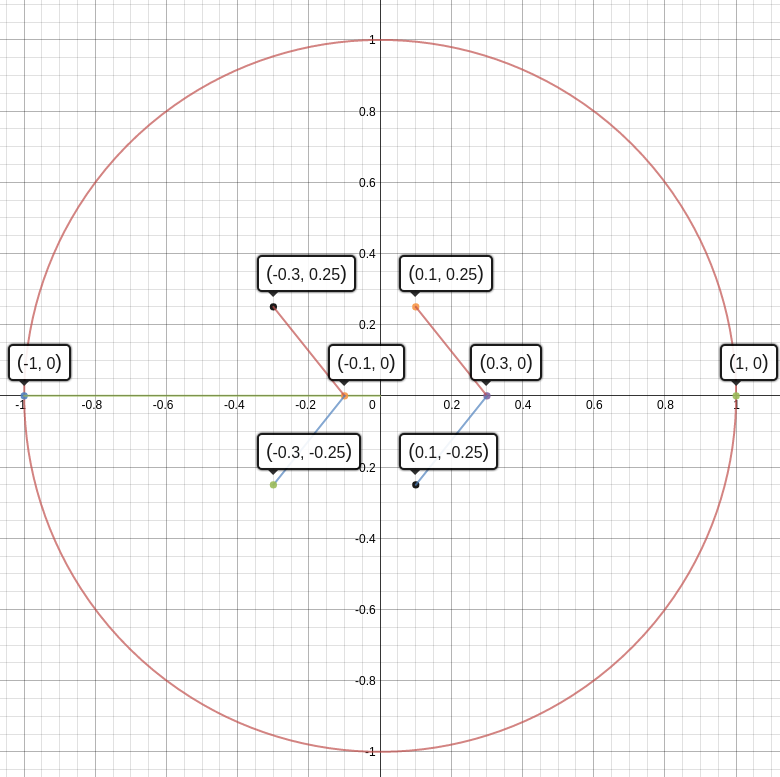
\includegraphics[scale=0.35]{graph_1}
\caption{Schita simbolului}
\label{fig:figura3}      
\end{figure}

\subsection{Sursa ideala de tensiune (SIT)}
In mod analog sursei ideale de curent, singurele simboluri pentru sursele ideale de tensiune pot fi observate in Fig.\ref{fig:figura4} si Fig.\ref{fig:figura5}. 

\begin{figure}[h]
\begin{minipage}{0.5\textwidth}
\centering

\begin{circuitikz} 
\draw
	   (0, 0) 
       to[american voltage source] (4,0)
       ;
\end{circuitikz}
\caption{SIT: model american}

\label{fig:figura4}       
\end{minipage}
\begin{minipage}{0.5\textwidth}
\centering
\begin{circuitikz} 
\draw
	   (0, 0) 
       to[european voltage source] (4,0)
       ;
\end{circuitikz}
\caption{SIT: model european}
\label{fig:figura5}  
\end{minipage}
\end{figure}

Totusi, in Romania, simbolul folosit este reprezentat de o sageata intr-un cerc, varful sagetii reprezentand borna "+" a sursei. Ca \c{s}i in cazul SIC, am reusit sa definesc un simbol care sa fie in conformitate cu cele folosite cu preponderenta in tara noastra. Astfel, el arata in felul urmator:

\begin{center}
\begin{circuitikz} 
\draw (0, 0) to[romanianVoltageSource] (4,0);
\end{circuitikz}
\end{center}

De asemenea, se comporta la fel ca orice alt element \c{s}i in circuite, avand posibilitatea de a il aseza pe orizontala, verticala sau diagonala \c{s}i in acelasi timp de a ii adauga etichete.

\begin{center}
\begin{circuitikz} 
\draw (0, 0) 
      to[romanianVoltageSource, l=${e_1 = 4V}$, *-*] (4, 0)
      to[romanianVoltageSource, l=${e_3}$, *-*] (4, -4)
      (0, 0)
      to[european resistor] (4, -4)
      (4, 0)
      to[european resistor] (8, 0)
      to[romanianVoltageSource, l=${e_2 = 7V}$, *-*] (4, -4)
      ;
\end{circuitikz}
\end{center}


\section{Utilizarea noilor simboluri}
Pentru a putea folosi oricine simbolurile create mai sus, 'in folderul \textit{symbols} aferent acestui proiect am inclus un fi\c{s}ier \textit{romanianCircuitSymbols.tex} cu definitiile celor doua simboluri \c{s}i ale regi\c{s}trilor aferen'ti. Downloadati acest fisier si 'in continuare, pentru folosirea lor cat mai u\c{s}oara in cadrul proiectului, tot ce trebuie s'a face'ti este s'a scrie'ti \verb!\makeatletter

\pgf@circ@Rlen = \pgfkeysvalueof{/tikz/circuitikz/bipoles/length}
\def\TikzBipolePath#1#2{\pgf@circ@bipole@path{#1}{#2}}
\makeatother

\newlength{\ResUp} 
\newlength{\ResRight}

%%%%%%%%%%%%%%%%%%%%%%%%%%%%%%%%%%%%%%%%%%%%%%%%%%%%%%%%%%%%%%%%%%%%%%%%%%%%%%%%%%%%%%%%%%%%%
%%%%%%%%%%%%%%%%%%      Sursa de curent: simbol folosit in Romania    %%%%%%%%%%%%%%%%%%%%%%%
%%%%%%%%%%%%%%%%%%%%%%%%%%%%%%%%%%%%%%%%%%%%%%%%%%%%%%%%%%%%%%%%%%%%%%%%%%%%%%%%%%%%%%%%%%%%%

%Declaram dimensiunile initiale
\ctikzset{bipoles/romanianCurrentSource/height/.initial=.60}
\ctikzset{bipoles/romanianCurrentSource/width/.initial=.60}

%Definim noul simbol pentru SIC
\pgfcircdeclarebipole{} 
	%Offset pentru label-uri
	{\ctikzvalof{bipoles/romanianCurrentSource/height}}
	%Numele simbolului
	{romanianCurrentSource}
	%Dimensiunile "cutiei" in care va sta
	{\ctikzvalof{bipoles/romanianCurrentSource/height}}
	{\ctikzvalof{bipoles/romanianCurrentSource/width}}
	{
		%Stabilim grosimea standard a liniei pentru un element
		\pgfsetlinewidth{\pgfkeysvalueof{/tikz/circuitikz/bipoles/thickness}\pgfstartlinewidth}
		
		%Definim ancorele
		\pgfextracty{\ResUp}{\northeast}
		\pgfextractx{\ResRight}{\southwest}
		
		%Desenam cerculetul
		\pgfpathellipse{\pgfpointorigin}{\pgfpoint{0}{\ResUp}}{\pgfpoint{\ResRight}{0}}
		
		%Desenam prima sagetica; trebuie sa avem grija ca dupa ce desenam un segment,
		%urmatoarea linie va fi desenata relativ la capatul segmentului, nu fata de
		%origine, deci sunt necesare cateva repozitionari
		\pgfmoveto{\pgfpoint{1.0\ResRight}{0.0\ResUp}}   %Ne pozitionam in (-1, 0)
		\pgflineto{\pgfpoint{0.1\ResRight}{0.0\ResUp}}   %Desenam corpul sagetii
		\pgflineto{\pgfpoint{0.3\ResRight}{-0.25\ResUp}} %Desenam unul din capete
		\pgfmoveto{\pgfpoint{0.1\ResRight}{0.0\ResUp}}   %Ne pozitionam in (-0.1, 0)
	    \pgflineto{\pgfpoint{0.3\ResRight}{0.25\ResUp}}  %Desenam celalalt capat
		
		%Desenam ce-a de-a doua sagetica
		\pgfmoveto{\pgfpoint{-0.2\ResRight}{0.0\ResUp}}  %Ne pozitionam in (0.2, 0)
		\pgflineto{\pgfpoint{-1.0\ResRight}{0.0\ResUp}}  %Desenam corpul sagetii
		\pgfmoveto{\pgfpoint{0.0\ResRight}{0.25\ResUp}}  %Ne repozitionam
		\pgflineto{\pgfpoint{-0.2\ResRight}{0.0\ResUp}}  %Desenam unul din capete
		\pgflineto{\pgfpoint{0.0\ResRight}{-0.25\ResUp}} %Desenam celalat capat
		
		%Pentru desenare, sa folosim functia draw
		\pgfusepath{draw}
	}

%Ii definim un stil si o cale si...gata!
\def\romanianCurrentSourcepath#1{\TikzBipolePath{romanianCurrentSource}{#1}}
\tikzset{romanianCurrentSource/.style = {\circuitikzbasekey, /tikz/to path=\romanianCurrentSourcepath, l=#1}}

%%%%%%%%%%%%%%%%%%%%%%%%%%%%%%%%%%%%%%%%%%%%%%%%%%%%%%%%%%%%%%%%%%%%%%%%%%%%%%%%%%%%%%%%%%%%%
%%%%%%%%%%%%%%%%%%      Sursa de ctensiune: simbol folosit in Romania    %%%%%%%%%%%%%%%%%%%%
%%%%%%%%%%%%%%%%%%%%%%%%%%%%%%%%%%%%%%%%%%%%%%%%%%%%%%%%%%%%%%%%%%%%%%%%%%%%%%%%%%%%%%%%%%%%%

%Declaram dimensiunile initiale
\ctikzset{bipoles/romanianVoltageSource/height/.initial=.60}
\ctikzset{bipoles/romanianVoltageSource/width/.initial=.60}

%Definim noul simbol pentru SIT
\pgfcircdeclarebipole{}
	%Stabilim grosimea standard a liniei pentru un element
	{\ctikzvalof{bipoles/romanianVoltageSource/height}}
	%Numele simbolului
	{romanianVoltageSource}
	%Dimensiunile "cutiei" in care va sta
	{\ctikzvalof{bipoles/romanianVoltageSource/height}}
	{\ctikzvalof{bipoles/romanianVoltageSource/width}}
	{
		%Stabilim grosimea standard a liniei pentru un element
		\pgfsetlinewidth{\pgfkeysvalueof{/tikz/circuitikz/bipoles/thickness}\pgfstartlinewidth}
		
		%Definim ancorele
		\pgfextracty{\ResUp}{\northeast}
		\pgfextractx{\ResRight}{\southwest}
		
		%Desenam cerculetul
		\pgfpathellipse{\pgfpointorigin}{\pgfpoint{0}{\ResUp}}{\pgfpoint{\ResRight}{0}}
		
		%Desenam prima sagetica; trebuie sa avem grija ca dupa ce desenam un segment,
		%urmatoarea linie va fi desenata relativ la capatul segmentului, nu fata de
		%origine, deci sunt necesare cateva repozitionari
		\pgfmoveto{\pgfpoint{1.0\ResRight}{0.0\ResUp}}   %Ne pozitionam in (-1, 0)
		\pgflineto{\pgfpoint{-1.0\ResRight}{0.0\ResUp}}   %Desenam corpul sagetii
		\pgflineto{\pgfpoint{-0.7\ResRight}{-0.25\ResUp}} %Desenam unul din capete
		\pgfmoveto{\pgfpoint{-1.0\ResRight}{0.0\ResUp}}   %Ne pozitionam in (-0.1, 0)
	    \pgflineto{\pgfpoint{-0.7\ResRight}{0.25\ResUp}}  %Desenam celalalt capat
		
		%Pentru desenare, sa folosim functia draw
		\pgfusepath{draw}
	}
	\def\romanianVoltageSourcepath#1{\TikzBipolePath{romanianVoltageSource}{#1}}
%Ii stabilim un nume, un posibil label si...gata!
\tikzset{romanianVoltageSource/.style = {\circuitikzbasekey, /tikz/to path=\romanianVoltageSourcepath, l=#1}}! 'in preambul, iar la compilare, acestea vor fi preluate automat. 'In modul de desenare al circuitului, utiliza'ti \verb!to[romanianCurrentSource]! pentru generearea simbolului pentru sursa ideal'a de curent 'si \verb!to[romanianVoltageSource]! pentru sursa ideal'a de tensiune. Ad'augarea nodurilor personalizate 'si a etichetelor se poate efectua la fel ca 'si pentru restul elementelor. Nu uita'ti s'a include'ti \verb!\usepackage{tikz}! \c{s}i \verb!\usepackage{circuitikz}! pentru o func'tionare corect'a!

\end{document}
